\section{Cơ sở lâm sàng}
\label{sec:clinical}

\subsection{Định nghĩa và phân loại}

Xuất huyết não là tình trạng chảy máu bên trong hộp sọ. Theo quy ước, nó được
phân chia theo khoang giải phẫu, và cách phân chia này có ý nghĩa đối với bài
toán kỹ thuật bởi các phân nhóm khác nhau rõ rệt về hình thái, kích thước và độ
khó phát hiện.

\begin{table}[H]
\centering
\small
\begin{tabularx}{\textwidth}{@{}l l X@{}}
\toprule
\textbf{Phân nhóm} & \textbf{Vị trí} & \textbf{Đặc điểm hình ảnh} \\
\midrule
Xuất huyết trong nhu mô (IPH) & Trong mô não & Khối tăng đậm độ dạng tròn, thường kèm phù nề xung quanh; hay gặp nhất ở hạch nền trong xuất huyết do tăng huyết áp \\
Xuất huyết não thất (IVH) & Hệ thống não thất & Máu lắng đọng theo tư thế; thường là sự lan rộng của IPH \\
Xuất huyết dưới nhện (SAH) & Khoang dưới nhện & Dải tăng đậm độ mỏng chạy dọc các rãnh vỏ não và bể nền; là phân nhóm bị bỏ sót nhiều nhất \\
Tụ máu dưới màng cứng (SDH) & Giữa màng cứng và màng nhện & Khối tụ hình liềm vượt qua các đường khớp sọ; thể mạn tính có thể đồng đậm độ hoặc giảm đậm độ \\
Tụ máu ngoài màng cứng (EDH) & Giữa xương sọ và màng cứng & Khối tụ hai mặt lồi (hình thấu kính), không vượt qua đường khớp sọ \\
\bottomrule
\end{tabularx}
\caption{Các phân nhóm xuất huyết não và biểu hiện trên hình ảnh.}
\label{tab:subtypes}
\end{table}

Hệ quả thực tiễn đối với thiết kế hệ thống là hình ảnh phải được trình bày với
chất lượng đủ để phân biệt được các phân nhóm này. Riêng SAH biểu hiện dưới
dạng vùng tăng đậm độ mỏng, độ tương phản thấp, dễ nhầm với cấu trúc mạch máu
bình thường hoặc với nhiễu ảnh do xơ cứng chùm tia gần nền sọ, nên đây là phân
nhóm bị bỏ sót nhiều nhất khi đọc. Việc phân biệt giữa các phân nhóm mang ý
nghĩa lâm sàng quyết định, bởi hướng xử trí khác biệt sâu sắc giữa, chẳng hạn,
một khối tụ máu ngoài màng cứng cần phẫu thuật lấy máu tụ khẩn cấp và một khối
tụ máu dưới màng cứng mạn tính nhỏ được điều trị bảo tồn.

\subsection{Các phương thức chẩn đoán hình ảnh}

\textbf{CT không tiêm thuốc cản quang} là phương thức tuyến đầu \cite{greenberg2022guideline} và là đối tượng
mà nền tảng này hướng tới. Máu cấp tính tăng đậm độ so với nhu mô não do quá
trình co cục máu đông làm cô đặc protein haemoglobin, và chênh lệch đậm độ này
đo được trực tiếp bằng đơn vị Hounsfield (HU): xuất huyết cấp thường đo được
50--70~HU so với 20--40~HU của nhu mô bình thường. CT nhanh (một ca chụp sọ não
mất chưa tới một phút), sẵn có ở mọi bệnh viện Việt Nam từ tuyến tỉnh trở lên,
và chi phí thấp. Hạn chế của nó là đậm độ khối máu tụ giảm dần theo thời gian,
nên các khối tụ bán cấp và mạn tính trở nên đồng đậm độ với mô não và tương ứng
khó phát hiện hơn.

\textbf{MRI} cho độ nhạy vượt trội với các ổ xuất huyết nhỏ, bán cấp và mạn
tính, đặc biệt trên các chuỗi xung gradient-echo và susceptibility-weighted,
vốn phát hiện được các sản phẩm thoái giáng thuận từ của haemoglobin. Tuy vậy,
đây vẫn là phương thức tuyến hai trong bối cảnh cấp cứu: thời gian thu nhận ảnh
lâu hơn đáng kể, chỉ sẵn có ở các trung tâm lớn, và không phù hợp với bệnh nhân
huyết động không ổn định. Do đó, đề tài này ưu tiên CT nhưng vẫn giữ kiến trúc
độc lập với phương thức chụp.

\subsection{Kỹ thuật cửa sổ và hệ quả đối với lưu trữ ảnh}
\label{sec:windowing}

Ảnh CT lưu trữ các giá trị suy giảm tia trong một dải rộng hơn nhiều so với khả
năng hiển thị của bất kỳ màn hình nào và rộng hơn nhiều so với khả năng phân
biệt của mắt người. Vì vậy, khi đọc trên lâm sàng người ta áp dụng một
\emph{cửa sổ} (window), tức một ánh xạ tuyến tính từ một khoảng HU được chọn
sang các mức xám khả dụng, loại bỏ mọi giá trị nằm ngoài khoảng đó. Một cửa sổ
được xác định bởi tâm cửa sổ (level) $L$ và độ rộng cửa sổ $W$; một điểm ảnh có
giá trị suy giảm $x$ được ánh xạ sang cường độ hiển thị

\begin{equation}
    y = \operatorname{clip}\!\left(\frac{x - (L - W/2)}{W},\ 0,\ 1\right).
\end{equation}

Bác sĩ chẩn đoán hình ảnh khi đọc tìm xuất huyết thường xem xét ít nhất ba cửa
sổ: cửa sổ \emph{nhu mô não} ($L=40$, $W=80$) để đánh giá nhu mô, cửa sổ
\emph{dưới màng cứng} ($L=75$--$100$, $W=200$--$300$) để làm rõ các khối tụ sát
xương sọ vốn bị bão hoà trong cửa sổ nhu mô não, và cửa sổ \emph{xương}
($L=600$, $W=2800$) để phát hiện các đường vỡ xương kèm theo.

Hình~\ref{fig:windowing} minh hoạ định lượng vì sao cần nhiều cửa sổ. Với cùng
chênh lệch khoảng 30~HU giữa máu cấp và nhu mô não, cửa sổ nhu mô não tạo ra chênh
lệch cường độ hiển thị $\Delta \approx 0{,}375$ trên thang $[0,1]$, tức khoảng 96
trên 256 mức xám; cửa sổ dưới màng cứng còn $\Delta \approx 0{,}15$; còn cửa sổ
xương chỉ còn $\Delta \approx 0{,}011$, chưa tới ba mức xám, và khối máu tụ gần như
không phân biệt được với mô xung quanh. Ngược lại, cửa sổ nhu mô não bão hoà mọi
giá trị trên 80~HU thành màu trắng, nên không dùng được để đánh giá xương hay tách
một khối tụ sát xương sọ khỏi bản xương.

\begin{figure}[H]
\centering
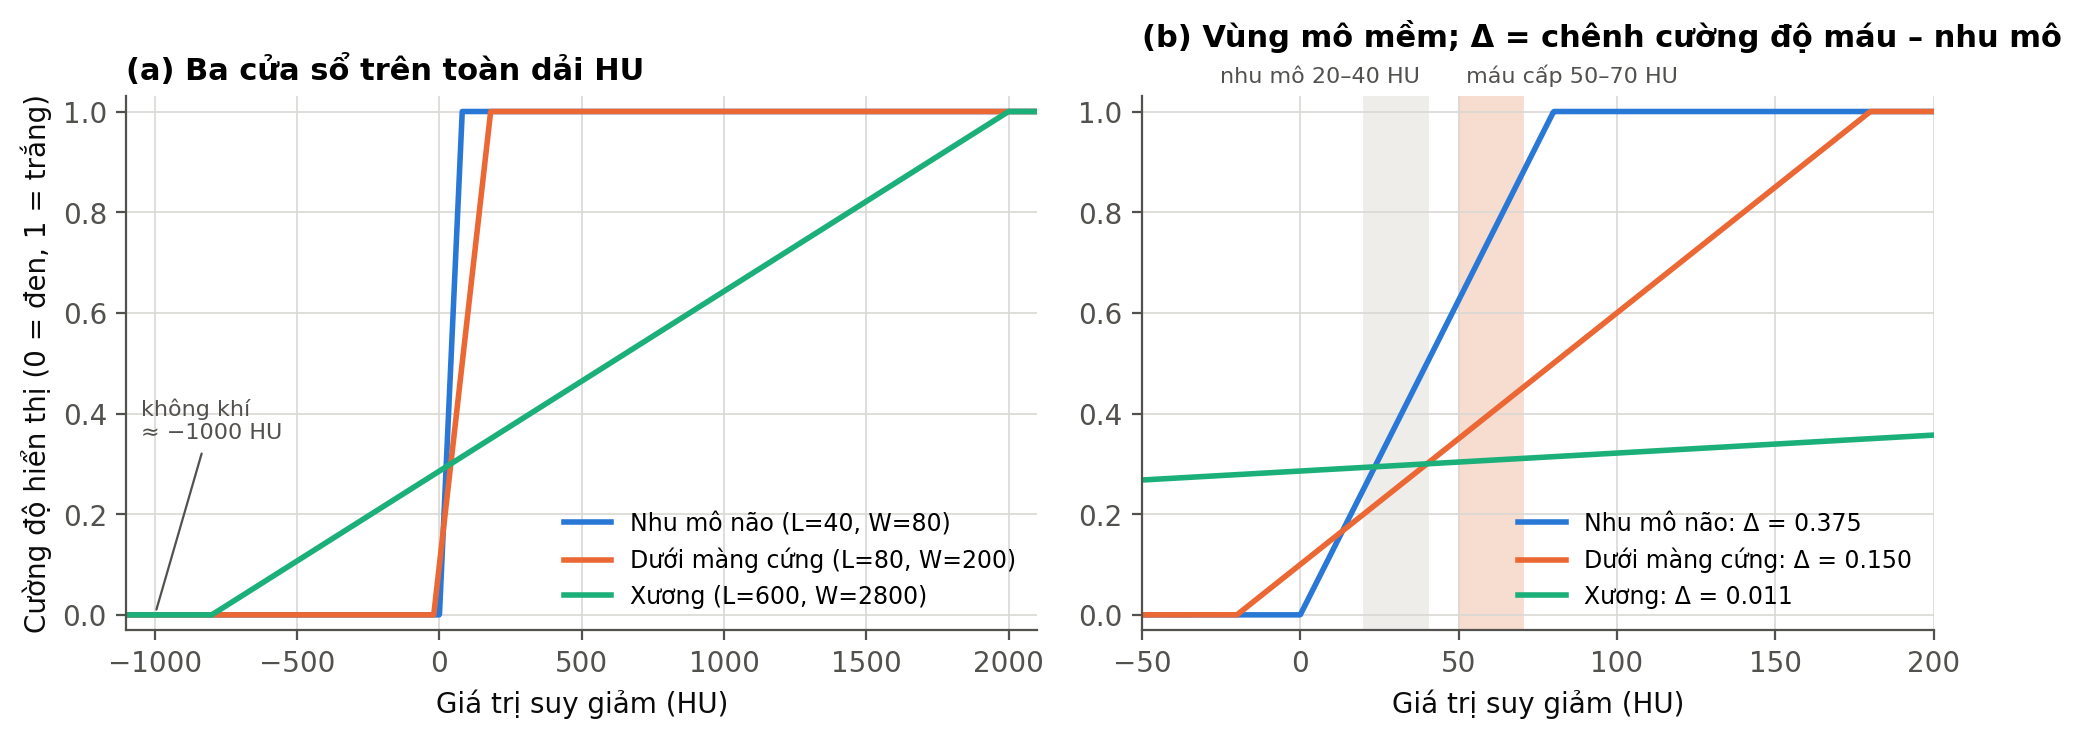
\includegraphics[width=\textwidth]{figures/fig_windowing.png}
\caption{Hàm ánh xạ cửa sổ hiển thị CT: (a) ba cửa sổ trên toàn dải HU; (b) phóng to
vùng mô mềm, với $\Delta$ là chênh lệch cường độ hiển thị giữa tâm vùng máu cấp
(60~HU) và tâm vùng nhu mô (30~HU). Mã nguồn: \texttt{figures/src/fig\_windowing.py}.}
\label{fig:windowing}
\end{figure}

Điều này dẫn tới một hệ quả kỹ thuật trực tiếp đối với cách lưu trữ dữ liệu. Vì
cửa sổ được chọn tuỳ theo điều bác sĩ đang tìm, hệ thống phải giữ nguyên dữ
liệu điểm ảnh DICOM gốc cùng các thuộc tính \texttt{RescaleSlope} và
\texttt{RescaleIntercept}, để trình xem có thể áp dụng bất kỳ cửa sổ nào tại
thời điểm đọc. Ngược lại, nếu lưu ảnh tám bit đã kết xuất sẵn thì quyết định
chọn cửa sổ đã được cố định một cách không thể đảo ngược, và bác sĩ mất khả
năng chuyển cửa sổ ngay trong lúc đọc.

\subsection{Quy trình lâm sàng và vai trò của nền tảng quản lý ảnh}

Một ca cấp tính điển hình diễn ra như sau. Bệnh nhân đến khoa cấp cứu; bác sĩ
chỉ định chụp CT sọ não; ca chụp được thực hiện trên thiết bị và truyền về
PACS; nó đi vào danh sách chờ đọc; một bác sĩ chẩn đoán hình ảnh đọc và ra kết
quả; bác sĩ điều trị xử trí dựa trên kết quả đó. Khoảng thời gian giữa lúc chụp
và lúc có kết quả chính là nơi độ trễ tích tụ, và một phần đáng kể độ trễ ấy
bắt nguồn từ khâu luân chuyển hình ảnh chứ không phải từ bản thân việc đọc.

Một nền tảng quản lý ảnh có thể rút ngắn chuỗi quy trình này ở những điểm sau:

\begin{itemize}
    \item \textbf{Truyền ảnh từ thiết bị về kho lưu trữ.} Ca chụp vừa hoàn tất
          được tự động chuyển về kho lưu trữ tập trung và sẵn sàng để đọc ngay,
          thay vì chờ thao tác thủ công tại máy trạm của thiết bị.
    \item \textbf{Truy cập hình ảnh từ nhiều vị trí.} Bác sĩ mở được ca chụp từ
          khoa phòng hoặc từ một máy tính bất kỳ trong bệnh viện, không nhất
          thiết phải có mặt tại phòng đọc chuyên dụng.
    \item \textbf{Đọc từ xa.} Khi cơ sở không có bác sĩ chẩn đoán hình ảnh tại
          chỗ, hình ảnh chuyển được tới bác sĩ ở nơi khác, điều này đặc biệt
          quan trọng ngoài giờ hành chính và ở tuyến dưới.
    \item \textbf{Loại bỏ khâu chuyển dữ liệu thủ công.} Việc ghi đĩa quang hay
          chép ổ đĩa di động để chuyển ảnh vừa chậm, vừa dễ thất lạc, vừa khó
          kiểm soát về mặt bảo mật.
\end{itemize}

Cần nhấn mạnh rằng nền tảng chỉ mang tính \emph{hỗ trợ}: nó cung cấp hình ảnh
và thông tin đi kèm một cách nhanh chóng và đầy đủ, chứ không đưa ra bất kỳ kết
luận nào. Chẩn đoán vẫn là hành vi của bác sĩ, phù hợp với quy định hành nghề
khám chữa bệnh của Việt Nam, theo đó chẩn đoán chỉ dành cho người có chứng chỉ
hành nghề. Do vậy, nền tảng phải được thiết kế sao cho mọi dữ liệu mà nó trình
bày đều truy được nguồn gốc và có thể đối chiếu lại với bản gốc.
